\documentclass[man]{apa6}

\usepackage{amssymb,amsmath}
\usepackage{ifxetex,ifluatex}
\usepackage{fixltx2e} % provides \textsubscript
\ifnum 0\ifxetex 1\fi\ifluatex 1\fi=0 % if pdftex
  \usepackage[T1]{fontenc}
  \usepackage[utf8]{inputenc}
\else % if luatex or xelatex
  \ifxetex
    \usepackage{mathspec}
    \usepackage{xltxtra,xunicode}
  \else
    \usepackage{fontspec}
  \fi
  \defaultfontfeatures{Mapping=tex-text,Scale=MatchLowercase}
  \newcommand{\euro}{€}
\fi
% use upquote if available, for straight quotes in verbatim environments
\IfFileExists{upquote.sty}{\usepackage{upquote}}{}
% use microtype if available
\IfFileExists{microtype.sty}{\usepackage{microtype}}{}

% Table formatting
\usepackage{longtable, booktabs}
\usepackage{lscape}
% \usepackage[counterclockwise]{rotating}   % Landscape page setup for large tables
\usepackage{multirow}		% Table styling
\usepackage{tabularx}		% Control Column width
\usepackage[flushleft]{threeparttable}	% Allows for three part tables with a specified notes section
\usepackage{threeparttablex}            % Lets threeparttable work with longtable

% Create new environments so endfloat can handle them
% \newenvironment{ltable}
%   {\begin{landscape}\begin{center}\begin{threeparttable}}
%   {\end{threeparttable}\end{center}\end{landscape}}

\newenvironment{lltable}
  {\begin{landscape}\begin{center}\begin{ThreePartTable}}
  {\end{ThreePartTable}\end{center}\end{landscape}}

  \usepackage{ifthen} % Only add declarations when endfloat package is loaded
  \ifthenelse{\equal{\string man}{\string man}}{%
   \DeclareDelayedFloatFlavor{ThreePartTable}{table} % Make endfloat play with longtable
   % \DeclareDelayedFloatFlavor{ltable}{table} % Make endfloat play with lscape
   \DeclareDelayedFloatFlavor{lltable}{table} % Make endfloat play with lscape & longtable
  }{}%



% The following enables adjusting longtable caption width to table width
% Solution found at http://golatex.de/longtable-mit-caption-so-breit-wie-die-tabelle-t15767.html
\makeatletter
\newcommand\LastLTentrywidth{1em}
\newlength\longtablewidth
\setlength{\longtablewidth}{1in}
\newcommand\getlongtablewidth{%
 \begingroup
  \ifcsname LT@\roman{LT@tables}\endcsname
  \global\longtablewidth=0pt
  \renewcommand\LT@entry[2]{\global\advance\longtablewidth by ##2\relax\gdef\LastLTentrywidth{##2}}%
  \@nameuse{LT@\roman{LT@tables}}%
  \fi
\endgroup}


  \usepackage{graphicx}
  \makeatletter
  \def\maxwidth{\ifdim\Gin@nat@width>\linewidth\linewidth\else\Gin@nat@width\fi}
  \def\maxheight{\ifdim\Gin@nat@height>\textheight\textheight\else\Gin@nat@height\fi}
  \makeatother
  % Scale images if necessary, so that they will not overflow the page
  % margins by default, and it is still possible to overwrite the defaults
  % using explicit options in \includegraphics[width, height, ...]{}
  \setkeys{Gin}{width=\maxwidth,height=\maxheight,keepaspectratio}
\ifxetex
  \usepackage[setpagesize=false, % page size defined by xetex
              unicode=false, % unicode breaks when used with xetex
              xetex]{hyperref}
\else
  \usepackage[unicode=true]{hyperref}
\fi
\hypersetup{breaklinks=true,
            pdfauthor={},
            pdftitle={Child language experience in a Tseltal Mayan village},
            colorlinks=true,
            citecolor=blue,
            urlcolor=blue,
            linkcolor=black,
            pdfborder={0 0 0}}
\urlstyle{same}  % don't use monospace font for urls

\setlength{\parindent}{0pt}
%\setlength{\parskip}{0pt plus 0pt minus 0pt}

\setlength{\emergencystretch}{3em}  % prevent overfull lines


% Manuscript styling
\captionsetup{font=singlespacing,justification=justified}
\usepackage{csquotes}
\usepackage{upgreek}

 % Line numbering
  \usepackage{lineno}
  \linenumbers


\usepackage{tikz} % Variable definition to generate author note

% fix for \tightlist problem in pandoc 1.14
\providecommand{\tightlist}{%
  \setlength{\itemsep}{0pt}\setlength{\parskip}{0pt}}

% Essential manuscript parts
  \title{Child language experience in a Tseltal Mayan village}

  \shorttitle{Child language experience in a Tseltal Mayan village}


  \author{Marisa Casillas\textsuperscript{1}, Penelope Brown\textsuperscript{1}, \& Stephen C. Levinson\textsuperscript{1}}

  % \def\affdep{{"", "", ""}}%
  % \def\affcity{{"", "", ""}}%

  \affiliation{
    \vspace{0.5cm}
          \textsuperscript{1} Max Planck Institute for Psycholinguistics  }

  \authornote{
    Correspondence concerning this article should be addressed to Marisa
    Casillas, P.O. Box 310, 6500 AH Nijmegen, The Netherlands. E-mail:
    \href{mailto:Marisa.Casillas@mpi.nl}{\nolinkurl{Marisa.Casillas@mpi.nl}}
  }


  \abstract{Enter abstract here. Each new line herein must be indented, like this
line.}
  \keywords{Child-directed speech, Linguistic input, Non-WEIRD, Vocal maturity, Turn
taking \\

    \indent Word count: X
  }





\usepackage{amsthm}
\newtheorem{theorem}{Theorem}[section]
\newtheorem{lemma}{Lemma}[section]
\theoremstyle{definition}
\newtheorem{definition}{Definition}[section]
\newtheorem{corollary}{Corollary}[section]
\newtheorem{proposition}{Proposition}[section]
\theoremstyle{definition}
\newtheorem{example}{Example}[section]
\theoremstyle{definition}
\newtheorem{exercise}{Exercise}[section]
\theoremstyle{remark}
\newtheorem*{remark}{Remark}
\newtheorem*{solution}{Solution}
\begin{document}

\maketitle

\setcounter{secnumdepth}{0}



\section{Introduction}\label{intro}

A great deal of work in developmental language science revolves around
one central question: What linguistic evidence (i.e., what types and how
much) is needed to support first language acquisition? In pursuing this
topic, many researchers have fixed their sights on child-directed speech
(CDS), showing that it is linguistically distinctive
(REFS)\textbf{{[}TASK 00: Add missing references{]}}, interactionally
rich (REFS), preferred by infants (REFS), and---perhaps most
importantly---facilitates word learning (REFS). One might then conclude
that CDS is an essential component for acquiring a first language. Yet
ethnographic reports from a number of traditional, non-Western
communities suggest that children easily acquire their community's
language(s) with little or no CDS (REFS). If so, CDS may not be
essential for learning language; just useful for facilitating certain
aspects of language development. In this paper we investigate the
language environment and early development of 10 Tseltal Mayan children
growing up in a community that reportedly uses very little CDS with
infants and young children (REFS Brown).

\subsection{Child-directed speech}\label{intro-cds}

The amount of CDS children hear influences their language development,
particularly their vocabulary (REFS). For example, \textbf{{[}TASK 01:
Add examples of input-vocab link{]}}. CDS has also been linked to young
children's speed of lexical retrieval (REFS Weisleder; LuCiD) and
syntactic development (REFS Huttenlocher). \textbf{{[}TASK 02: Read
Huttenlocher and add details here{]}}. The conclusion drawn from much of
this work is that CDS is an ideal register for learning
words---especially concrete nouns and verbs---because it is tailored to
maximize a child's moment-to-moment interest and understanding (REFS).
Indeed, even outside of first-person interaction, infants and young
children prefer listening to CDS over adult-directed speech (REFS
ManyBabies, etc.), suggesting that CDS is useful in catching,
maintaining, and focusing children's attention. There are, however, a
few significant caveats to the body of work relating CDS quantity to
language development.

First, while there is overwhelming evidence linking CDS quantity to
vocabulary size, links to grammatical development are more scant (REFS:
Huttenlocher; Frank et al.). Children must master the systemic
underpinnings of their language(s), e.g., the phonology, morphology, and
syntax. While the advantage of CDS for referential word learning is
clear, it is less obvious how CDS facilitates syntactic learning.
\textbf{{[}TASK 03: Add argument from Yurovsky paper + refrences
therein{]}} On the other hand, there is a wealth of evidence that both
children and adults' syntactic knowledge is highly lexically specified
(REFS), and that, crosslinguistically, children's vocabulary size is one
of the most robust predictors of their early syntactic development
(REFS). In short, what is good for the lexicon may also be good for
syntax. For now, however, the link between CDS and other aspects of
grammatical development still needs to be more thoroughly tested.

Second, \textbf{{[}TASK 04: Add paragraph on burstiness{]}}

Third, prior work has typically focused on Western (primarily North
American) populations, limiting our ability to generalize these effects
to children acquiring language worldwide (REFS: WEIRD; Lieven, 1994).
While we do gain valuable insight by looking at \emph{within-population}
variation (e.g., REFS), we can more effectively find places where our
assumptions break down by studying \emph{new} populations. Linguistic
anthropologists working in non-Western communities have long reported
that caregiver interaction styles vary immensely from place to place,
with some caregivers using little or no CDS to young children (REFS
Gaskins, 2006). Children in these communities reportedly acquire
language with \enquote{typical}-looking benchmarks. For example, they
start pointing (REFS Liszkowski) and talking (REFS Rogoff et al., 2003?;
Brown??) around the same time we would expect for Western middle-class
infants. These findings have had little impact on mainstream theories of
word learning and language acquisition, partly due to a lack of directly
comparable measures (Brown, 2014). If, however, these children indeed
acquire language without delay despite little or no CDS, we must
reconsider what kind of linguistic evidence is necessary for children to
learn language.

\subsection{Language development in non-WEIRD
communities}\label{intro-nonweird}

To our knowledge, only a handful of researchers have used methods from
developmental psycholinguistics to describe the language environments
and linguistic development of children growing up in traditional,
non-Western communities. We focus here on \emph{quantitative} language
development measures because the key claims about CDS and linguistic
development are themselves quantitative in nature. We briefly highlight
two recent efforts along these lines, but see Cristia et al. (2017) for
a recent review.

Scaff, Cristia, and colleagues (REFS 2017; in preparation) have used a
number of methods to estimate how much speech children hear in a Tsimane
forager-horticulturalist population in the Bolivian lowlands. Their
daylong recordings show that Tsimane children between 0;6 and 6;0 hear
\textasciitilde{}5 minutes of CDS per hour, with no increase for older
children (but see Cristia et al., 2017). For comparison, children from
North American homes between ages 0;3 and 3;0 are estimated to hear
\textasciitilde{}11 minutes of CDS per hour in daylong recordings (REFS:
Bergelson, Casillas, et al., see also REFS the newer Tamis-LeMonda
paper; maybe give estimates w/ age ranges for each??). In addition to
CDS, Tsimane children also hear \textasciitilde{}10 minutes of
other-directed speech per hour (e.g., talk between adults)---more than
the \textasciitilde{}7 minutes of adult-directed speech per hour North
American children are estimated to hear (REFS Bergelson, Casillas, et
al.). This difference may be attributable to the fact that the Tsimane
live in extended family clusters of 3--4 households, and so speakers are
typically in close proximity to 5--8 other people (REFS Cristia et al.,
2017).

Laura Shneidman and colleagues (REFS; 2010; 2012) analyzed speech from
1-hour at-home video recordings of children between ages 1;0 and 3;0 in
two communities: Yucatec Mayan (Southern Mexico) and North American (in
a major US city). Their analyses yielded four main findings: compared to
the American children, (a) the Yucatec children heard many fewer
utterances per hour, (b) a much smaller proportion of the utterances
they heard were \emph{child-directed}, (c) the proportion of utterances
that were child-directed increased dramatically with age, matching U.S.
children's by 3;0 months, and (d) most of the added CDS came from other
children (e.g., older siblings and cousins). They also demonstrated that
the lexical diversity of the CDS they hear at 24 months---particularly
from adult speakers---predicted children's vocabulary knowledge at 35
months.

These groundbreaking studies establish a number of important findings:
First, children in each of these communities appear able to acquire
their languages with relatively little CDS. Second, CDS may become more
frequent as children get older, though this may be largely due to speech
from other children. Finally, despite these differences, CDS from adults
may still be the most robust predictor of vocabulary growth.

\subsection{The current study}\label{intro-currentstudy}

We examine the early language experience of 10 Tseltal Mayan children
under age 3;0. Prior ethnographic work suggests that Tseltal caregivers
do not frequently speak directly to their children until the children
themselves begin speaking (REFS: Brown??). Nonetheless, Tseltal children
develop language with no apparent delays. Tseltal Mayan language and
culture has much in common with the Yucatec Mayan communities Shneidman
has worked with (REFS: 2010 + add other stuff that's not nec lg), which
allows us to compare differences in child language environments between
the two sites more directly than before.\textbackslash{}footnote\{For a
review of comparative work in developmental linguistic anthropology,
particularly on Mayan cultures, see Pye (2017).) We provide more details
on this community and dataset in the \protect\hyperlink{methods}{Methods
section}.

Similar to previous work by Shneidman, Scaff, Cristia, and colleages, we
estimated how much speech children overheard, how much was directed to
them, and how those quantities changed with age. To this foundation we
added new sampling techniques for investigating variability in
children's speech environments within daylong recordings. We also
analyzed children's early vocal productions, examining both the overall
developmental trajectory of their vocal maturity and how their
vocalizations are influenced by CDS.

Based on prior work, we predicted that Tseltal Mayan children hear
little CDS, that the amount of CDS they hear increases with age, that
most CDS comes from other children, and that, despite this, Tseltal
Mayan children would hit early speech production benchmarks on par with
Western children. We additionally predicted that children's language
environments would be bursty---that brief, high-intensity interactions
would be sparsely distributed throughout the day, accounting for the
majority of children's daily CDS---and that children's responsiveness
and vocal maturity would be maximized during these moments of
high-intensity interaction.

\hypertarget{methods}{\section{Methods}\label{methods}}

\subsection{Community}\label{methods-community}

The children in our dataset (REFS: Casillas HomeBank) come from a
small-scale, subsistence farming community in the highlands of Chiapas
in Southern Mexico. The vast majority of children grow up speaking
Tseltal monolingually at home. Primary school is conducted in Tseltal,
but secondary and further education is primarily conducted in Spanish.
Nuclear families are often large (5+ children) and live in patrilineal
clusters. Nearly all families grow staple crops such as corn and beans,
but also bananas, chilies, squash, and coffee. Families also cultivate
and collect a range of other local plants, raise poultry for eggs and
meat and, very occasionally, raise other animals (e.g., bulls) for
slaughter. Additional produce, meat, and processed foods are available
for purchase at small local shops and from vendors driving through town.
Household and farming work is divided among men, women, and older
children. Women do much of the daily cleaning and food preparation, but
also frequently work in the garden, haul water and firewood, and do
other physical labor. A few community members---both men and
women---earn incomes as teachers and shopkeepers but are still expected
to regularly contribute to their family's household work.

Based on more than forty years of fieldwork in this community, the
second author has characterized Tseltal children's language environments
as non-child-centered. During their waking hours, Tseltal infants are
typically tied to their mother's back while she goes about her work for
the day. Infants receive very little direct speech until they themselves
begin to initiate interactions as they near their first birthday. Even
then, interactional exchanges are often brief or non-verbal (e.g.,
object exchange routines) and most often take place within a
multi-participant---non-dyadic---context (Brown 2011; 2014). Rarely is
attention given to words and their meanings, even when objects are
central to the activity. Instead, interactions tend to focus on
appropriate actions and responses, and young children are socialized to
attend to the interactions taking place around them (REFS). Young
children are often cared for by other family members, especially older
siblings, and are rarely put down on the ground before they are ready to
start walking, so they rarely have the opportunity to independently pick
up objects before age 1;0. Even so, toys are scarce and books are
vanishingly rare, so the objects children do get their hands on tend to
be natural or quotidien objects with clear functions in daily life
(e.g., spoons, baskets, etc.). By age five, most children are competent
speakers who engage in chores and caregiving of their younger siblings.
This caregiving approach is similar to those described for other Mayan
communities (e.g., REFS Rogoff, Gaskins, de Leon, Shneidman).

\subsection{Corpus and data selection}\label{methods-corpus}

\begin{itemize}
\tightlist
\item
  fertility info
\item
  carrying info
\item
  info on older sibling caregivers Extended households in our dataset
  (defined as those who share a kitchen or other primary living space)
  ranged between between 3 and 15 people \emph{{[}TASK 06: Check this
  range{]}}. 
\end{itemize}

\subsection{How to define temporal contingency for turn
taking}\label{how-to-define-temporal-contingency-for-turn-taking}

Many other studies of child-caregiver turn taking use an arbitrary
cut-off for detecting contingency (5 seconds?? Look up references). We
base ours on measures of turn taking in interactions with infants and
young children. Hilbrink et al. (2015) looked at interaction in a
longitudinal corpus from 3 to 18 months and found that infants'
responses to mothers began between -700ms and 1200ms relative to the end
of the mothers' turns. Complementarily, mothers' responses to infant
vocalizations began between -350ms and 650ms relative to the end of the
infants' turns. Casillas et al. (2016) investigated the timing of
question-answer responses from caregiver to child and from child to
caregiver with children between 20 and 35 months. In their study,
children's responses typically started between -500ms and 650ms relative
to the end of their caregivers' turns. Caregivers' responses typically
started between -1000ms and 400ms relative to the end of their
children's turns. Because both studies focused on fairly intensive bouts
of interaction, and both within WEIRD parental contexts, we defined
contingent responses in the current data with slightly generous
allowances for overlap and gap: contingent responses must begin with no
more than 1000ms of overlap and 2000ms of gap relative to the offset of
the first speaker's turn. We used this same criteria for finding
child-to-other turn transitions and other-to-child turn transitions.
Transitions were only counted if the other speaker's turn was coded as
addressed to \enquote{T} (the target child).

\subsection{Data analysis}\label{methods-analysisinfo}

\section{Results}\label{results}

\subsection{Still to graph}\label{still-to-graph}

3: sliding window in random to match mean TDS rate/TT transition rates
4: utt length, repetitiveness, F0 peaks and ranges

\subsection{SHOULD I ADD DATAPOINTS ON THE UPH FIGS TO SHOW SHNEIDMAN'S
DATA?}\label{should-i-add-datapoints-on-the-uph-figs-to-show-shneidmans-data}

Age 1: - US: CDS 616 (SD=231); ADS/OCDS 278 (SD=247) -- 79\% XDS from
MOT (\textasciitilde{}60\% XDS MOT is CDS); 8\% XDS from children
(mostly ADS/OCDS) - Mayan: CDS 86 (SD=59); ADS/OCDS 342 (SD=201) -- 31\%
XDS from MOT (\textasciitilde{}4\% XDS MOT is CDS); 60\% XDS from
children (\textasciitilde{}50\% XDS other kids was ADS/OCDS) Age18mo?:
Age 2: - US: CDS M=815, SD=376; ADS/OCDS M=411, SD=318 -- M=65\%,
SD=28\% from MOT (directed: M=800, SD=381; overheard: M=211, SD =55); --
M=7\%, SD=10\% from kids (directed: M=15, SD=22; overheard: M=86,
SD=141) - Mayan: CDS M=274, SD=166; ADS/OCDS M=271, SD=136 -- M=19\%,
SD=17\% from MOT (directed:M=104, SD=100; overheard:M=82 SD=52); --
M=61\%, SD=27\% from kids (directed:M=104, SD=100; overheard:M=82 SD=52)
Age35mo?

\subsubsection{Observation only data}\label{observation-only-data}

13 months Directed speech 140 (55); Overheard speech 377 (176) 18 months
Directed speech 211 (70); Overheard speech 240 (96) 24 months Directed
speech 315 (69); Overheard speech 360 (73) (I think these data weren't
coded for adult vs.~child speaker)

\begin{figure}
\centering
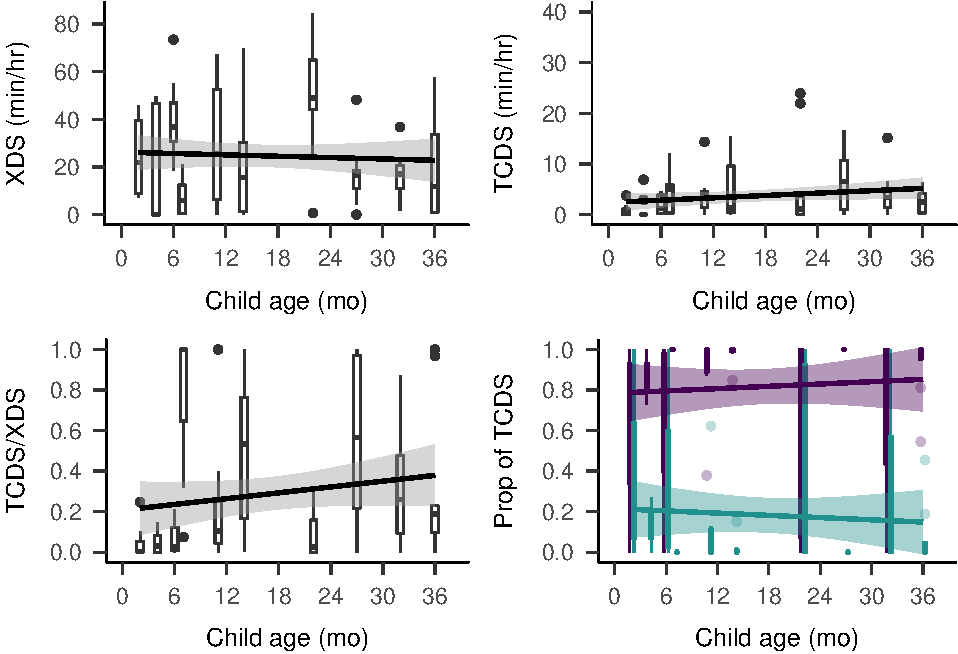
\includegraphics{Tseltal-CLE_files/figure-latex/plot_XDS_TDS_quantity_random-1.pdf}
\caption{}
\end{figure}

\begin{figure}
\centering
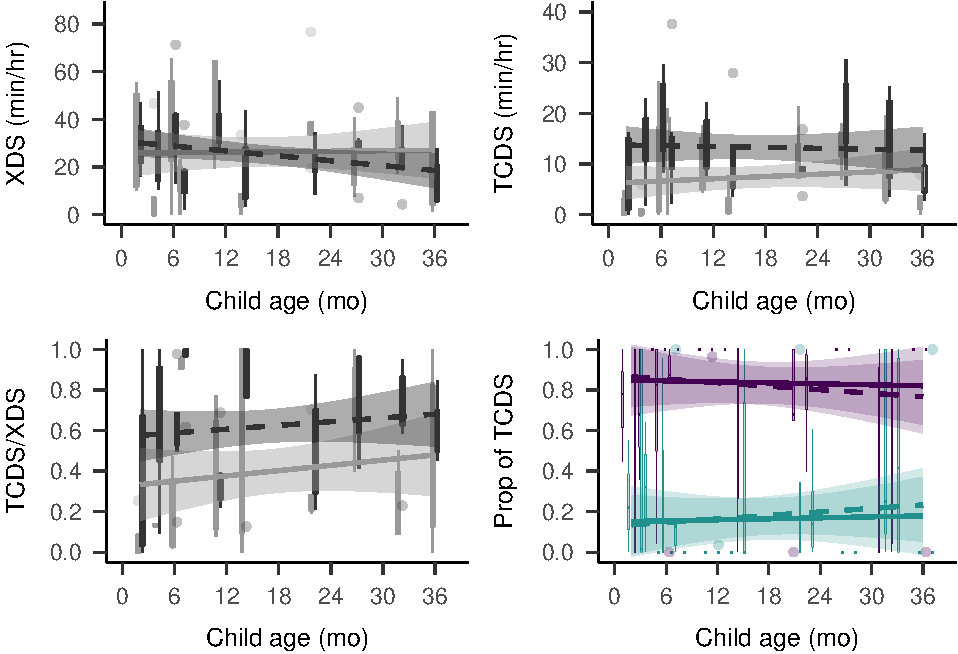
\includegraphics{Tseltal-CLE_files/figure-latex/plot_XDS_TDS_quantity_nonrandom-1.pdf}
\caption{}
\end{figure}

\begin{figure}
\centering
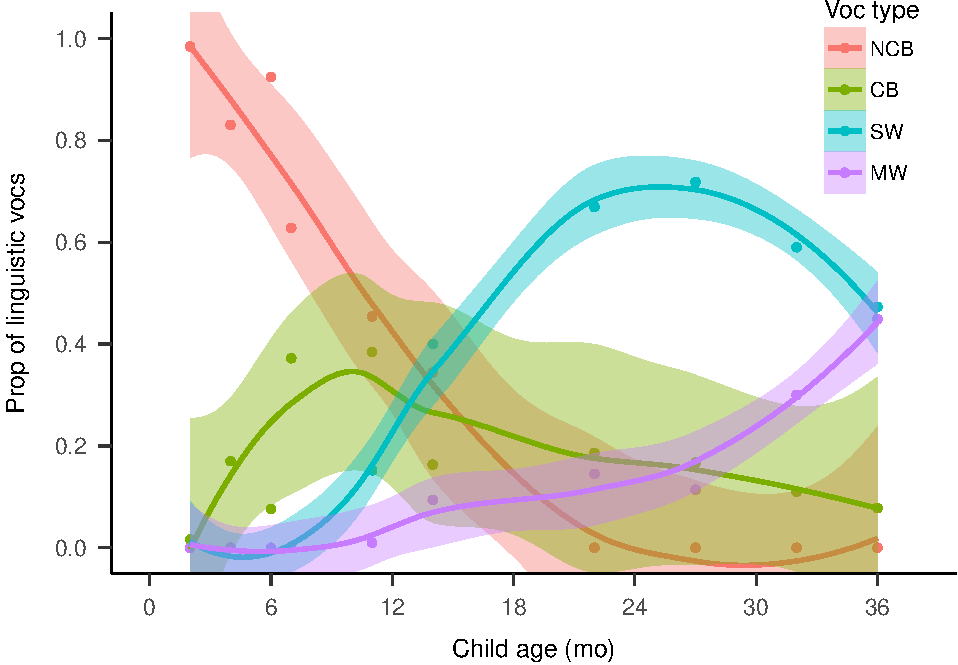
\includegraphics{Tseltal-CLE_files/figure-latex/plot_chi_voctypes_overall-1.pdf}
\caption{}
\end{figure}

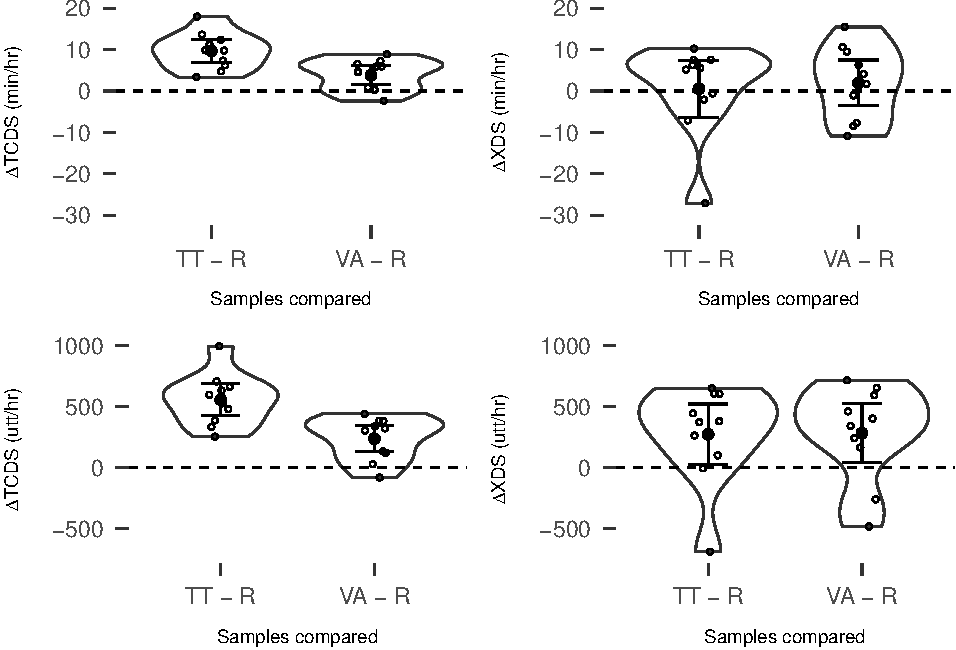
\includegraphics{Tseltal-CLE_files/figure-latex/plot_sample_differences-1.pdf}
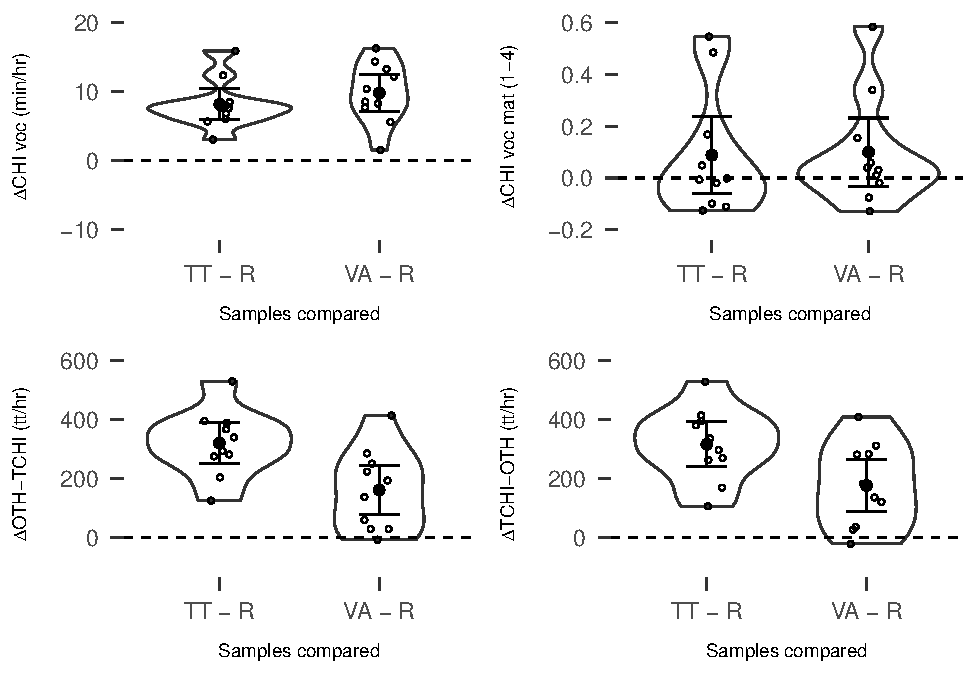
\includegraphics{Tseltal-CLE_files/figure-latex/plot_sample_differences-2.pdf}

\section{Discussion}\label{disc}

\subsection{Future directions}\label{disc-future}

\subsection{Conclusion}\label{disc-conclusion}

\newpage

\section{References}\label{refs}

\begingroup
\setlength{\parindent}{-0.5in} \setlength{\leftskip}{0.5in}

\hypertarget{refs}{}

\endgroup






\end{document}
